\begin{frame}
	\frametitle{Herramientas y Tecnologías utilizadas}
	\block{ Android Studio}
		\begin{itemize}
			\item Entorno de desarrollo integrado.
			\item Gradle.
			\item Sistema de depuración sencillo e intuitivo.
		\end{itemize}
		Descarga en: \texttt{https://developer.android.com/studio/index.html}
	\endblock{}
\end{frame}

%------------------------------------------------------------------
\begin{frame}
	\frametitle{Herramientas y Tecnologías utilizadas}
	\block{\it Realidad Aumentada}
		\begin{itemize}
			\item {\it ¿Qué es la Realidad Aumentada?}.
			\item {\it ¿Cómo funciona esta tecnología?}.
			\item {\it ¿Qué tipos de Realidad Aumentada existen?}.
			\item {\it ¿En qué se diferencia la Realidad Aumentada con la Realidad Virtual?}.
			\item {\it ¿Qué futuro le espera a la Realidad Aumentada?}.
			\item {\it Integración de la Realidad Aumentada en Android Studio}.
		\end{itemize}
	\endblock{}
\end{frame}

%------------------------------------------------------------------

\begin{frame}
	\frametitle{Herramientas y Tecnologías utilizadas}
	\begin{columns}
		\begin{column}{0.6\textwidth}
			\block{\it ¿Qué es la realidad aumentada?}
			\begin{itemize}
				\item Pequeño dispositivo que emite señales utilizando Bluetooth.
				\item Señales unidireccionales que emiten información.
				\item Recibidas por dispositivos móviles.
				\item Aplicaciones programadas para recibir estas señales.
			\end{itemize}
			\endblock{}
		\end{column}
		\begin{column}{0.4\textwidth}
			\vfill 
			\begin{center}
				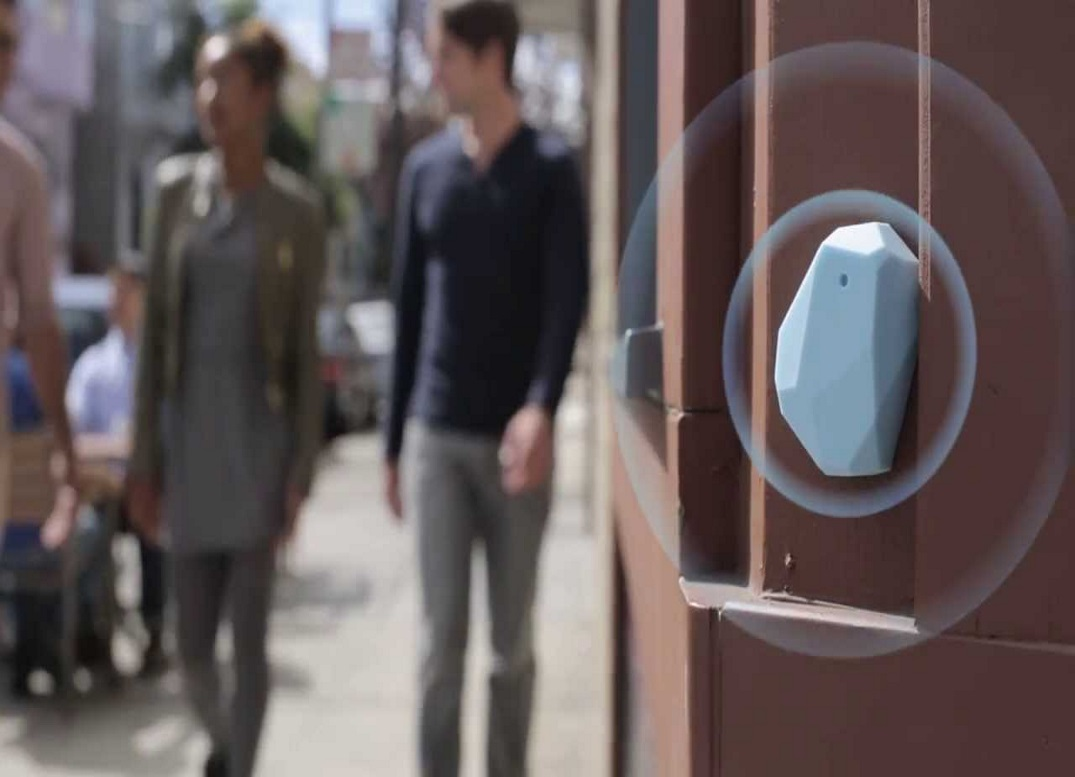
\includegraphics[width=0.8\linewidth]{Images/estimoteBeacon}
			\end{center}
		\end{column}
	\end{columns}
\end{frame}

%------------------------------------------------------------------
\begin{frame}
	\frametitle{Herramientas y Tecnologías utilizadas}
		\begin{columns}
			\begin{column}{0.6\textwidth}
				\block{\it ¿Cómo funciona esta tecnología?}
					\begin{itemize}
						\item {Los beacons usan Bluetooth Low Energy (BLE).}
						\item {Los beacons funcionan con baterías.}
						\item {Transmiten identificadores cortos.}
					\end{itemize}
				\endblock{}
			\end{column}
			\begin{column}{0.4\textwidth}
				\vfill 
					\begin{center}
						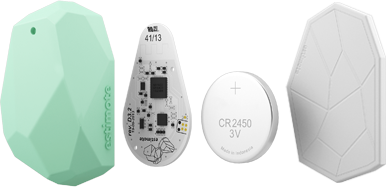
\includegraphics[width=0.8\linewidth]{Images/estimoteBeaconInside}
					\end{center}
			\end{column}
		\end{columns}
\end{frame}		
		


\begin{frame}
	\frametitle{Herramientas y Tecnologías utilizadas}
	\begin{columns}
			\begin{column}{0.6\textwidth}
				\block{\it ¿Qué tipos de Realidad Aumentada existen?}
					\begin{itemize}
						\item {Rango de 70 m de radio sin obstáculos.}
						\item {Este rango puede disminuir signicativamente.}
						\item {Las aplicaciones suelen definir acciones en tres rangos.}
						\item {Es posible lanzar acciones a una distancia determinada.}
					\end{itemize}
				\endblock{}
			\end{column}
			\begin{column}{0.4\textwidth}
				\vfill 
					\begin{center}
						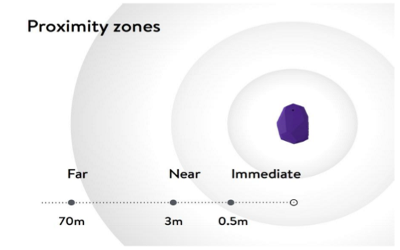
\includegraphics[width=0.95\linewidth]{Images/beaconsRange}
					\end{center}
			\end{column}
	\end{columns}
\end{frame}

%------------------------------------------------------------------

\begin{frame}
	\frametitle{Herramientas y Tecnologías utilizadas}
	\begin{columns}
			\begin{column}{0.6\textwidth}
				\block{\it ¿En qué se diferencia la Realidad Aumentada con la Realidad Virtual?}
					\begin{itemize}
						\item {Todos los dispositivos que soporten BLE.}
						\item {En IOS7 o superior.}
						\item {En dispositivos Android.}
					\end{itemize}
				\endblock{}
			\end{column}
			\begin{column}{0.4\textwidth}
				\vfill 
					\begin{center}
						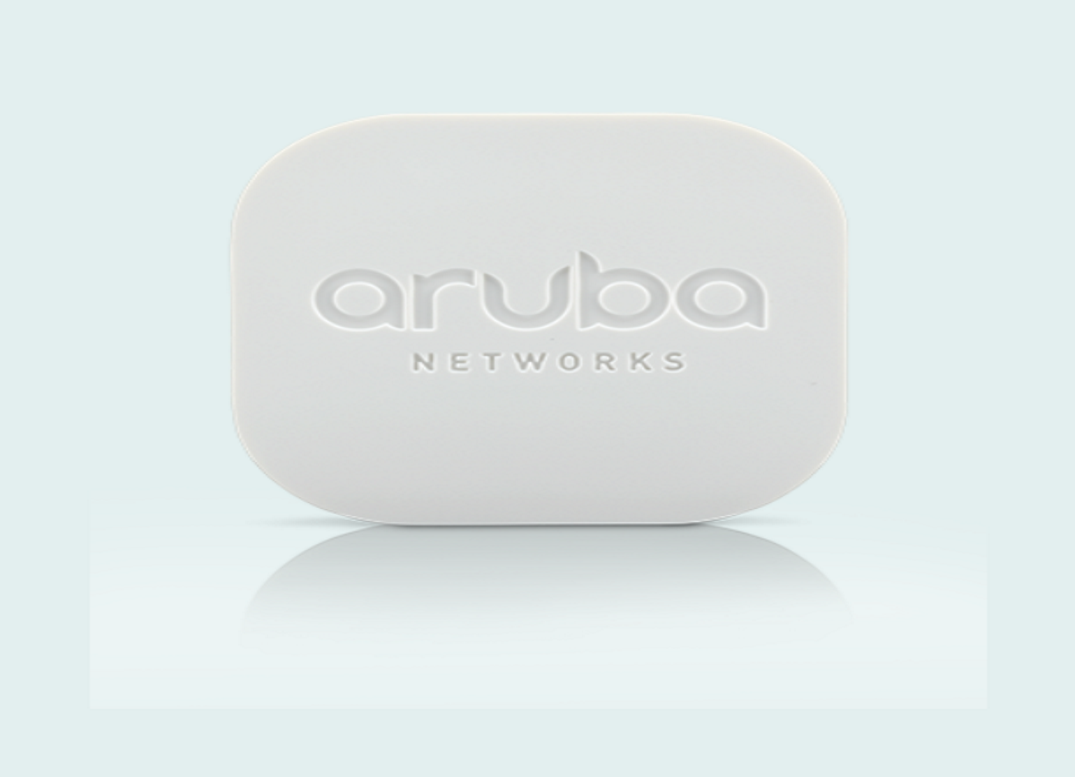
\includegraphics[width=0.8\linewidth]{Images/arubaBeacons}
					\end{center}
			\end{column}
	\end{columns}
\end{frame}

%--------------------------------------------------------------------

\begin{frame}
	\frametitle{Herramientas y Tecnologías utilizadas}
	\block{\it ¿Qué futuro le espera a la Realidad Aumentada?}
		\begin{columns}
			\begin{column}{0.9\textwidth}
				\block{\it Ventajas}
					\begin{itemize}
						\item {BLE menos batería que GPS.}
						\item {Funciona en el interior de los edificios.}
					\end{itemize}
				\endblock{}			
				\block{\it Desventajas}
					\begin{itemize}
						\item {Dependen de aplicaciones instaladas.}
						\item {Es necesario activar el Bluetooth.}
						\item {Su utilidad depende de la voluntad de terceros.}
					\end{itemize}
				\endblock{}
			\end{column}
		\end{columns}
	\endblock{}
\end{frame}


\begin{frame}
	\frametitle{Herramientas y Tecnologías utilizadas}
	\block{\it  Integración de la Realidad Aumentada en Android Studio}
		\begin{columns}
			\begin{column}{0.3\textwidth}
				Clevedon School App
				\vspace{3mm}
				\vfill 
					\begin{center}
						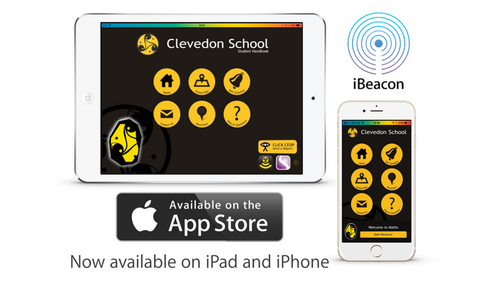
\includegraphics[width=0.8\linewidth]{Images/ClevedonApp}
					\end{center}
			\end{column}
			\begin{column}{0.3\textwidth}
				Levi's Stadium App
				\vspace{3mm}
				\vfill 
					\begin{center}
						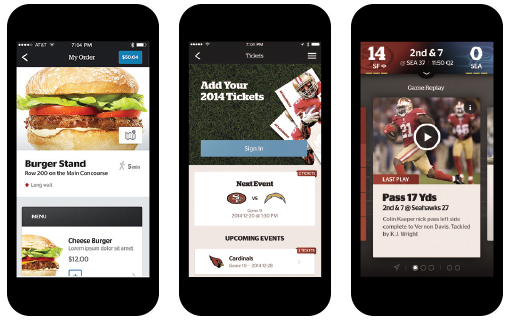
\includegraphics[width=0.8\linewidth]{Images/LevisStadium}
					\end{center}
			\end{column}
			\begin{column}{0.3\textwidth}
				Orlando Int'l Airport
				\vspace{3mm}
				\vfill 
					\begin{center}
						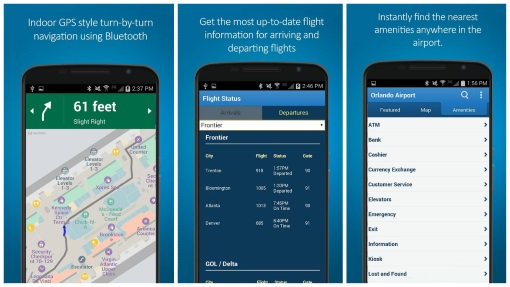
\includegraphics[width=0.8\linewidth]{Images/orlandoAirport}
					\end{center}
			\end{column}
		\end{columns}
	\endblock{}
\end{frame}

\begin{frame}
	\frametitle{Herramientas y Tecnologías utilizadas}
		\block{\it Node.js}
			\begin{itemize}
				\item {¿Qué es?}
				\item {¿Qué nos ha permitido?}
				\item {¿Por qué se ha decidido utilizar esta tecnología?}
			\end{itemize}
		\endblock{}
		\vfill 
			\begin{center}
				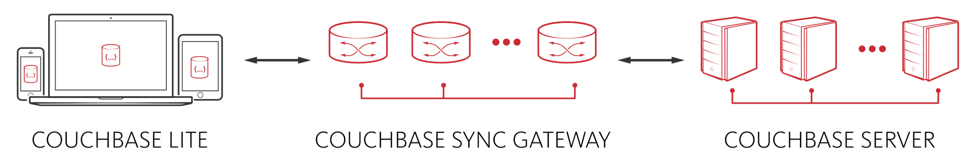
\includegraphics[width=1\linewidth]{Images/couchBase}
			\end{center}
\end{frame}

\begin{frame}
	\frametitle{Herramientas y Tecnologías utilizadas}
		\block{\it MongoDB}
			Se puede definir AltBeacon como una especificación que:
			\begin{itemize}
				\item {Define el formato del protocolo publicitario a través de BLE.}
				\item {Intenta crear un mercado abierto y competitivo para implementaciones utilizando proximidad.}
				\item {Puede ser utilizada gratuitamente, sin cuotas ni compromisos.}
				\item {No favorece a ningún proveedor sobre otro.}
			\end{itemize}
		\endblock{}
		\block{\it Funcionamiento}
			\begin{columns}
				\begin{column}{0.7\textwidth}
					\begin{itemize}
						\item {Monitorizacion(\textit{``Monitoring''})}
						\item {Rastreo (\textit{``Ranging''})}
					\end{itemize}
				\end{column}
				\begin{column}{0.3\textwidth}
					\vfill 
					\begin{center}
						
\includegraphics[width=0.5\linewidth]{Images/logos/altBeacon}
					\end{center}
				\end{column}
			\end{columns}
		\endblock{}
\end{frame}

\begin{frame}
	\frametitle{Herramientas y Tecnologías utilizadas}
	\begin{columns}
			\begin{column}{0.6\textwidth}
				\block{\it Heroku}
					\begin{itemize}
						\item {Es un método matemático para determinar las posiciones relativasde objetos.}
						\item {Utiliza las localizaciones de dos o más puntos y las distancias entre el sujeto y cada punto.}
						\item {En un plano bidimensional, se necesitan al menos tres puntos de referencia.}
					\end{itemize}
				\endblock{}
			\end{column}
			\begin{column}{0.4\textwidth}
				\vfill 
					\begin{center}
						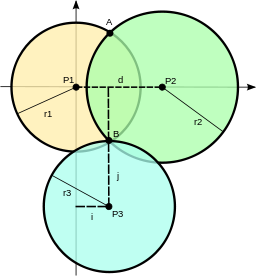
\includegraphics[width=0.8\linewidth]{Images/trilateration}
					\end{center}
			\end{column}
	\end{columns}
\end{frame}

\begin{frame}
	\frametitle{Herramientas y Tecnologías utilizadas}
	\begin{columns}
			\begin{column}{0.6\textwidth}
				\block{\it mLab}
					\begin{itemize}
						\item {Es un método matemático para determinar las posiciones relativasde objetos.}
						\item {Utiliza las localizaciones de dos o más puntos y las distancias entre el sujeto y cada punto.}
						\item {En un plano bidimensional, se necesitan al menos tres puntos de referencia.}
					\end{itemize}
				\endblock{}
			\end{column}
			\begin{column}{0.4\textwidth}
				\vfill 
					\begin{center}
						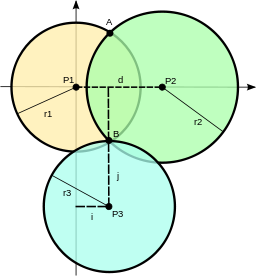
\includegraphics[width=0.8\linewidth]{Images/trilateration}
					\end{center}
			\end{column}
	\end{columns}
\end{frame}

\begin{frame}
	\frametitle{Herramientas y Tecnologías utilizadas}
	\begin{columns}
			\begin{column}{0.6\textwidth}
				\block{\it Google Maps}
					\begin{itemize}
						\item {Es un método matemático para determinar las posiciones relativasde objetos.}
						\item {Utiliza las localizaciones de dos o más puntos y las distancias entre el sujeto y cada punto.}
						\item {En un plano bidimensional, se necesitan al menos tres puntos de referencia.}
					\end{itemize}
				\endblock{}
			\end{column}
			\begin{column}{0.4\textwidth}
				\vfill 
					\begin{center}
						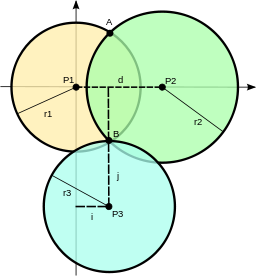
\includegraphics[width=0.8\linewidth]{Images/trilateration}
					\end{center}
			\end{column}
	\end{columns}
\end{frame}

%--------------------------------------------------------------------
